\documentclass{article}

% if you need to pass options to natbib, use, e.g.:
%     \PassOptionsToPackage{numbers, compress}{natbib}
% before loading neurips_2023

% ready for submission
\usepackage[final]{neurips_2023}

% to avoid loading the natbib package, add option nonatbib:
%    \usepackage[nonatbib]{neurips_2023}

\usepackage[utf8]{inputenc} % allow utf-8 input
\usepackage[T1]{fontenc}    % use 8-bit T1 fonts
\usepackage{hyperref}       % hyperlinks
\usepackage{url}            % simple URL typesetting
\usepackage{booktabs}       % professional-quality tables
\usepackage{amsfonts}       % blackboard math symbols
\usepackage{nicefrac}       % compact symbols for 1/2, etc.
\usepackage{microtype}      % microtypography
\usepackage{xcolor}         % colors
\usepackage{graphicx}       % images
\usepackage{subcaption}
\usepackage{wrapfig}
\usepackage{siunitx}
\usepackage{amsmath}
\usepackage{listings}

\graphicspath{{images}}

\title{Task 3: Data Exploration}
\author{% 
  Team Vectorized Engines \AND
  Simon Grundner (k12136610)
  \And
  Mihael Zupanic (k12416041)
}


\begin{document}

\maketitle

\section{Verification of Annotations and Qualitative Analysis}

\subsection{Summary of Disagreements}

\begin{itemize}
    \item Minor changes were made in a few annotations which correctly recognized the class but did not capture the whole length of the event.
    \item Cut a few audio events which had excessive margin to length.
    \item In an event where a glass was put under a coffee machine and then started, the annotator thought that the description did not fit the scene and incorrectly classified unidentifiable rustling noises as handling glassware and coffee machine noises.
    \item Audio event labeled \emph{window\_open\_close} was corrected to \emph{door\_open\_close} as described in the scene description.
    \item Annotation was fixed by adding the completely missing events from the target class footsteps.
\end{itemize}

\subsection{Case Study: Clear violation of the annotation rules}

A violation of the annotation rules was found. The metadata of the scene are as follows

\begin{itemize}
    \item \textbf{Audio file:} \emph{000278.wav}
    \item \textbf{Scene description:} started clicking on a mouse and then a keyboard. slid chair, stood up, and slid the chair back. walked towards the phone and started dialing a number.
    \item \textbf{Target classes:} \emph{keyboard\_typing}, \emph{footsteps}
    \item \textbf{Non-target sounds:} \emph{mouse\_clicking}, \emph{sliding\_chair}, \emph{number\_dialing}
    \item \textbf{Environment:} office 
    \item \textbf{Placement:} mobile
\end{itemize}

\autoref{fig:case1-correct} shows the waveform with the correct annotation for the target classes, while \autoref{fig:case1-incorrect} completely misses the \emph{keyboard\_typing} section and also a few clearly audible footsteps. The second annotation also places the \emph{keyboard\_typing} class at the end of the scene, which is incorrect. The person in the scene dials a number on a phone with a dual tone dial system, which does not resemble keyboard strokes. The two tones from the phone dial can be clearly seen in the spectrum.

A reason for missing the keyboard sounds could be that the keyboard in the audio does not have a classic \emph{clicky} sound but a rather deep \emph{thumping} sound, which the annotator was maybe not familiar with.

Both parties left out footsteps between standing up from the chair and sliding the chair in. The fixed annotation in \autoref{fig:case1-accepted} marks the missed footsteps.


\begin{figure}
\centering
\begin{subfigure}[c]{\textwidth}
    \centering
    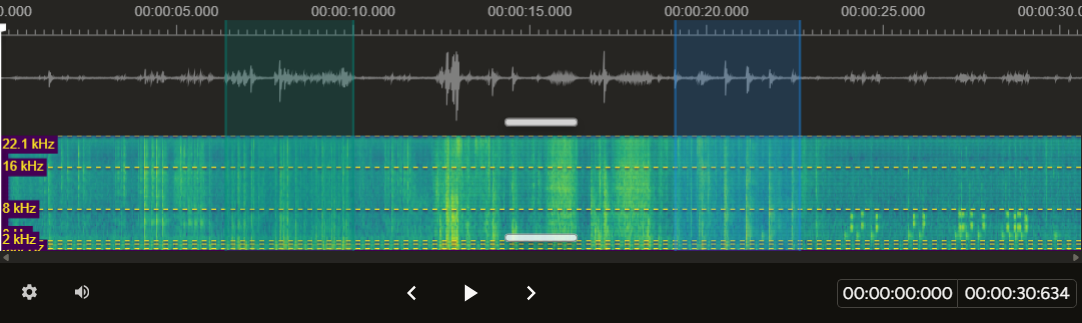
\includegraphics[width=0.6\linewidth]{Case1-moreCorrect}
    \subcaption{Annotation which fits the scene correctly. Here the keyboard typing (green), which is mentioned in the description and also clearly audible, as well as the footsteps (blue) are sectioned.}
    \label{fig:case1-correct}
\end{subfigure}
\medskip

\begin{subfigure}[c]{\textwidth}
    \centering
    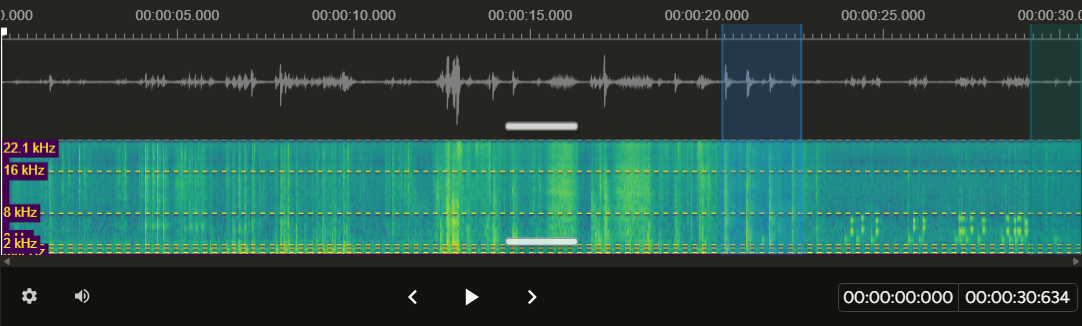
\includegraphics[width=0.6\linewidth]{Case1-lessCorrect}
    \subcaption{Annotation which misses the entire \emph{keyboard\_typing} (green) class and incorrectly puts it to the end of the file. The footsteps (blue) section is also shorter than in actual fact.}
    \label{fig:case1-incorrect}
\end{subfigure}
\medskip

\begin{subfigure}[c]{\textwidth}
    \centering
    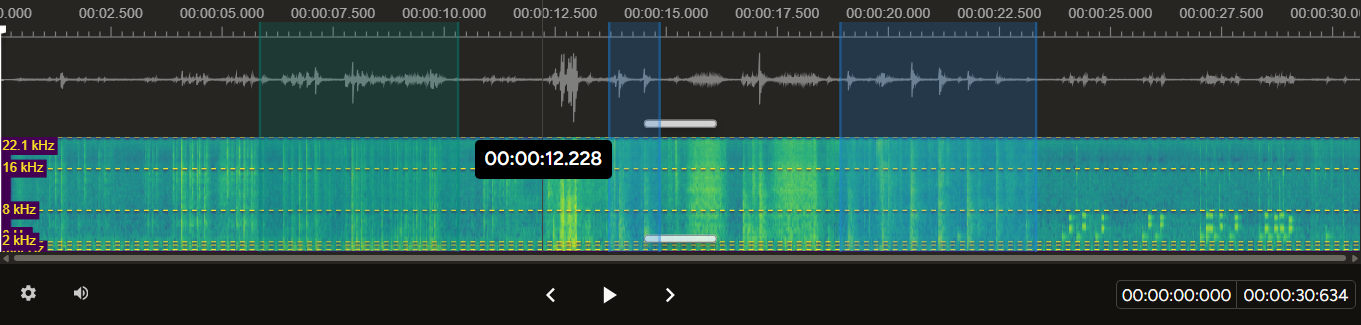
\includegraphics[width=0.6\linewidth]{Case1-acceptedVersion}
    \subcaption{Fixed annotation, which correctly applies the sections from the first original annotation and also two more clearly audible footsteps.}
    \label{fig:case1-accepted}
\end{subfigure}
\caption{Case Study of annotation rule violation}
\end{figure}

\newpage
\section{Annotations}

\subsection{Annotator Agreement}

We measured annotator agreement using the Jaccard index — the ratio of cells where all annotators agreed a sound was active (intersection) to cells where at least one annotator marked it active (union). Files with only one annotator (625 out of 3656) were excluded. For class-wise agreement, intersection and union counts were accumulated per class across all files.
The overall mean Jaccard is 71.0\% (std 22.5\%), indicating substantial agreement across recordings. As shown in the Figure 2, continuous sounds like vacuum\_cleaner (86.2\%) and keyboard\_typing (83.6\%) score highest, while brief events like door\_open\_close (52.3\%) and wardrobe\_drawer\_open\_close (51.9\%) score lowest. This suggests disagreement is driven more by uncertain onset/offset boundaries than by annotators missing sounds entirely. To verify this, we checked whether each target class tag specified by the collector appeared in at least one temporal annotation — 97.5\% of tags were confirmed, indicating that annotators found almost everything the collector intended to capture.

\begin{figure}
    \centering
    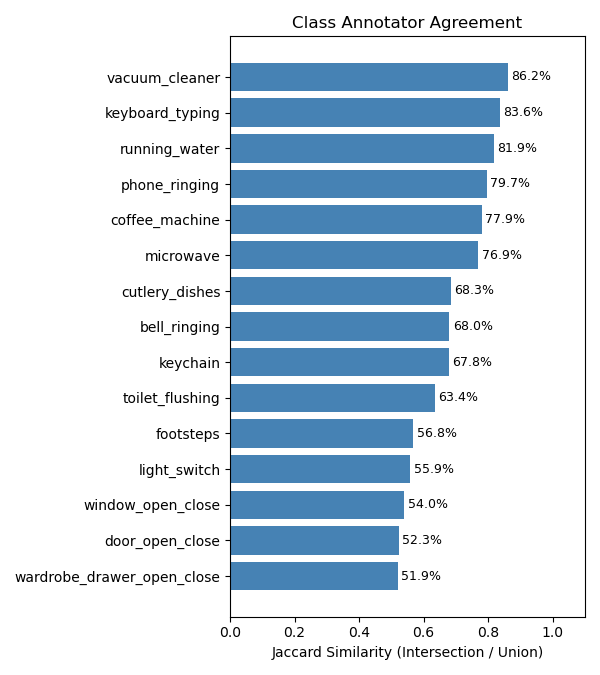
\includegraphics[width=0.4\textwidth]{images/fig_jaccard.png}
    \caption{Per-class annotator agreement measured by Jaccard Similarity (Intersection over Union)}\label{fig:jaccard}
    \hfill
\end{figure}
    
\subsection{Annotations to Labels Conversion}

The annotation array [T, C, A] contains overlap fractions (0 to 1) between each annotator's marked regions and each time segment. We convert this to a binary label matrix [T, C] in two steps: firstly, any overlap > 0 is counted as a yes vote from that annotator. Secondly, a cell becomes 1 if more than half of annotators voted yes. With two annotators both must agree, while for one annotator that vote decides alone.

We assume all annotators are equally trustworthy and don't give the collector more weight from the is\_own\_recording flag. We also don't use the collector's target\_classes tag as a label source. Quiet sounds where annotators disagree default to 0, therefore we are biased towards false negatives rather than false positives (hallucinating sounds that aren't there). Single-annotator files skipped the agreement check, so whatever the one annotator marked becomes the label.

\subsection{Label Characteristics}

As shown in Figure 3a, classes are greatly imbalanced — footsteps is the most common (2576 events) while coffee\_machine is the rarest (287 events). Duration (Figure 3b) shows a clear split between short events like light\_switch (median 1.5s) and long-running ones like vacuum\_cleaner (17.0s). This lines up with longer sounds having the highest Jaccard index.

Co-occurrence patterns match everyday house activities: door\_open\_close and footsteps (802 files), footsteps and keychain (441), footsteps and light\_switch (432). Other pairs link to specific rooms, like cutlery\_dishes and running\_water (363, kitchen), running\_water and toilet\_flushing (284, bathroom). We also checked class frequencies per recording environment — classes cluster by room, with only footsteps and door\_open\_close spread across all environments.

\begin{figure}[htb]
    \centering
    \begin{subfigure}[t]{0.49\textwidth}
        \centering
        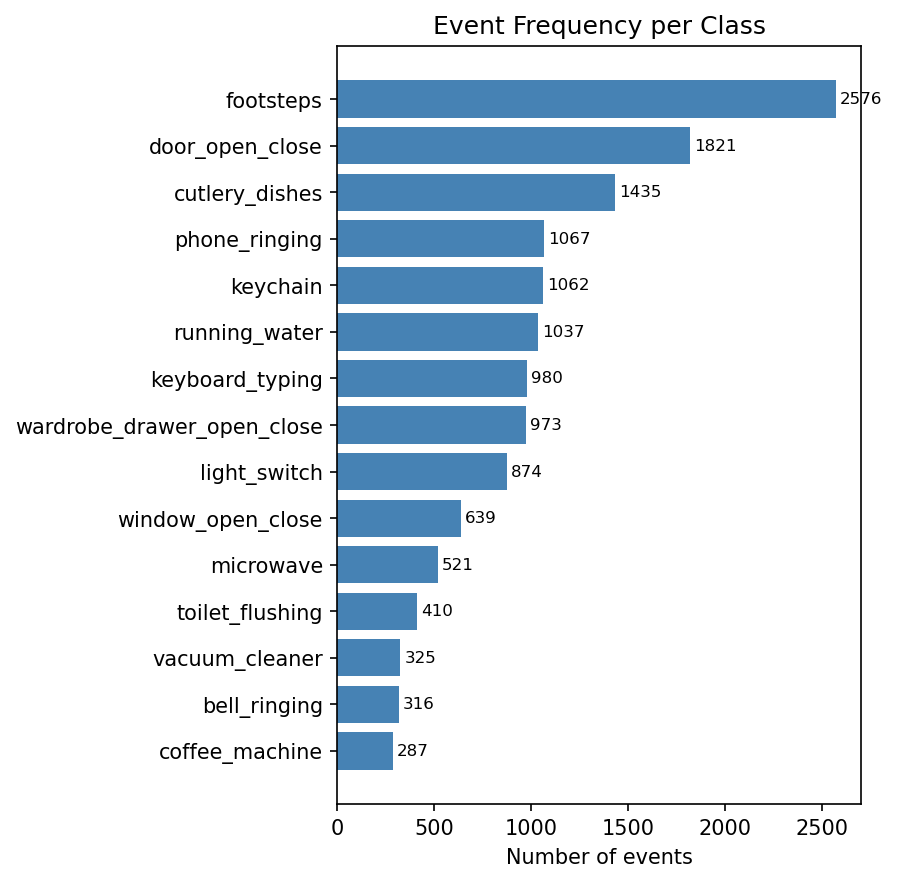
\includegraphics[width=\textwidth]{images/freq.png}
        \caption{Number of events per class across all files.}\label{fig:placement-freq}
    \end{subfigure}%
    \hfill
    \begin{subfigure}[t]{0.49\textwidth}
        \centering
        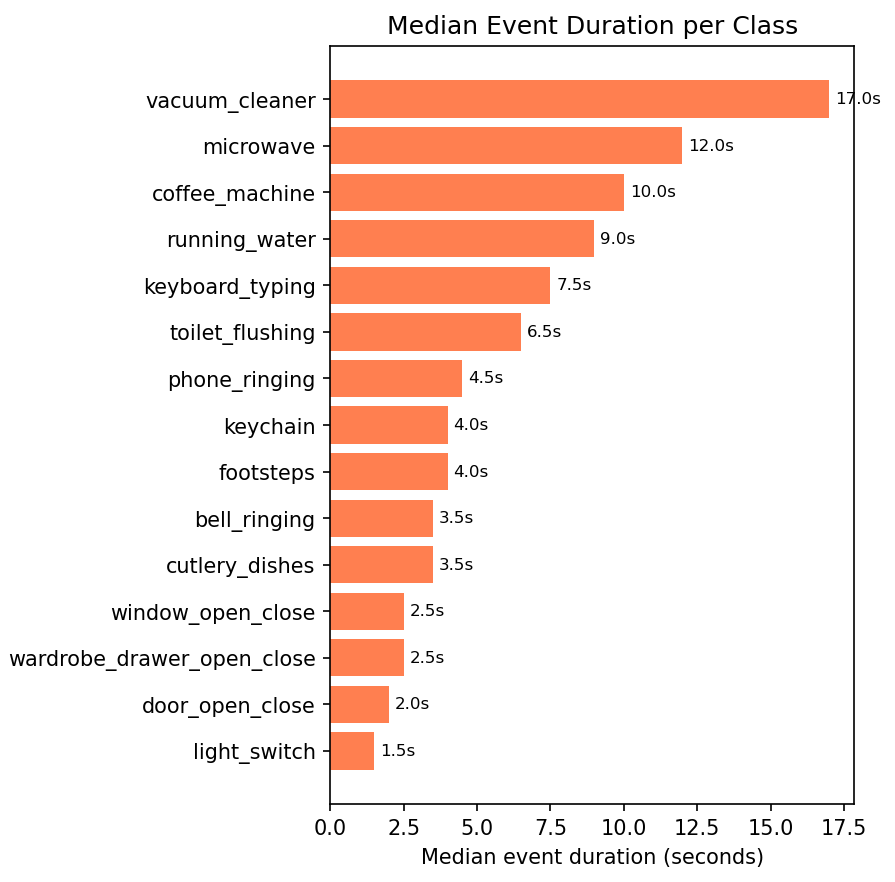
\includegraphics[width=\textwidth]{images/duration.png}
        \caption{Median event duration per class in seconds.}\label{fig:placement-duration}
    \end{subfigure}
    \caption{Class-wise event frequency and duration of the binary labels}\label{fig:bin-labels}
\end{figure}

\newpage
\section{Audio Features}

\subsection{Metadata Distribution}

The device placement was chosen as the property to be analyzed. \autoref{fig:device-placement} shows, which classes occur most for each device placement.
The dominant classes for \emph{mobile} recording devices can be seen in \autoref{fig:placement-mobile}. Here, the \emph{footsteps} class dominates by far, followed by \emph{door\_open\_close}. This might indicate that a room was entered in these scenarios.
\autoref{fig:placement-static} shows the dominant classes for \emph{static} recording devices. Here, the dominant classes occur in similar amounts. These classes are also from different categories of the household (e.g. \emph{keyboard\_typing} and \emph{cutlery\_dishes}), whereas classes for mobile placement seem more closely related (e.g. \emph{door\_open\_close} and \emph{keychain}) 

It seems that a static placement allowed for a wider variety of scenarios, compared to a mobile placement.

\begin{figure}[htb]
    \centering
    \begin{subfigure}[t]{0.49\textwidth}
        \centering
        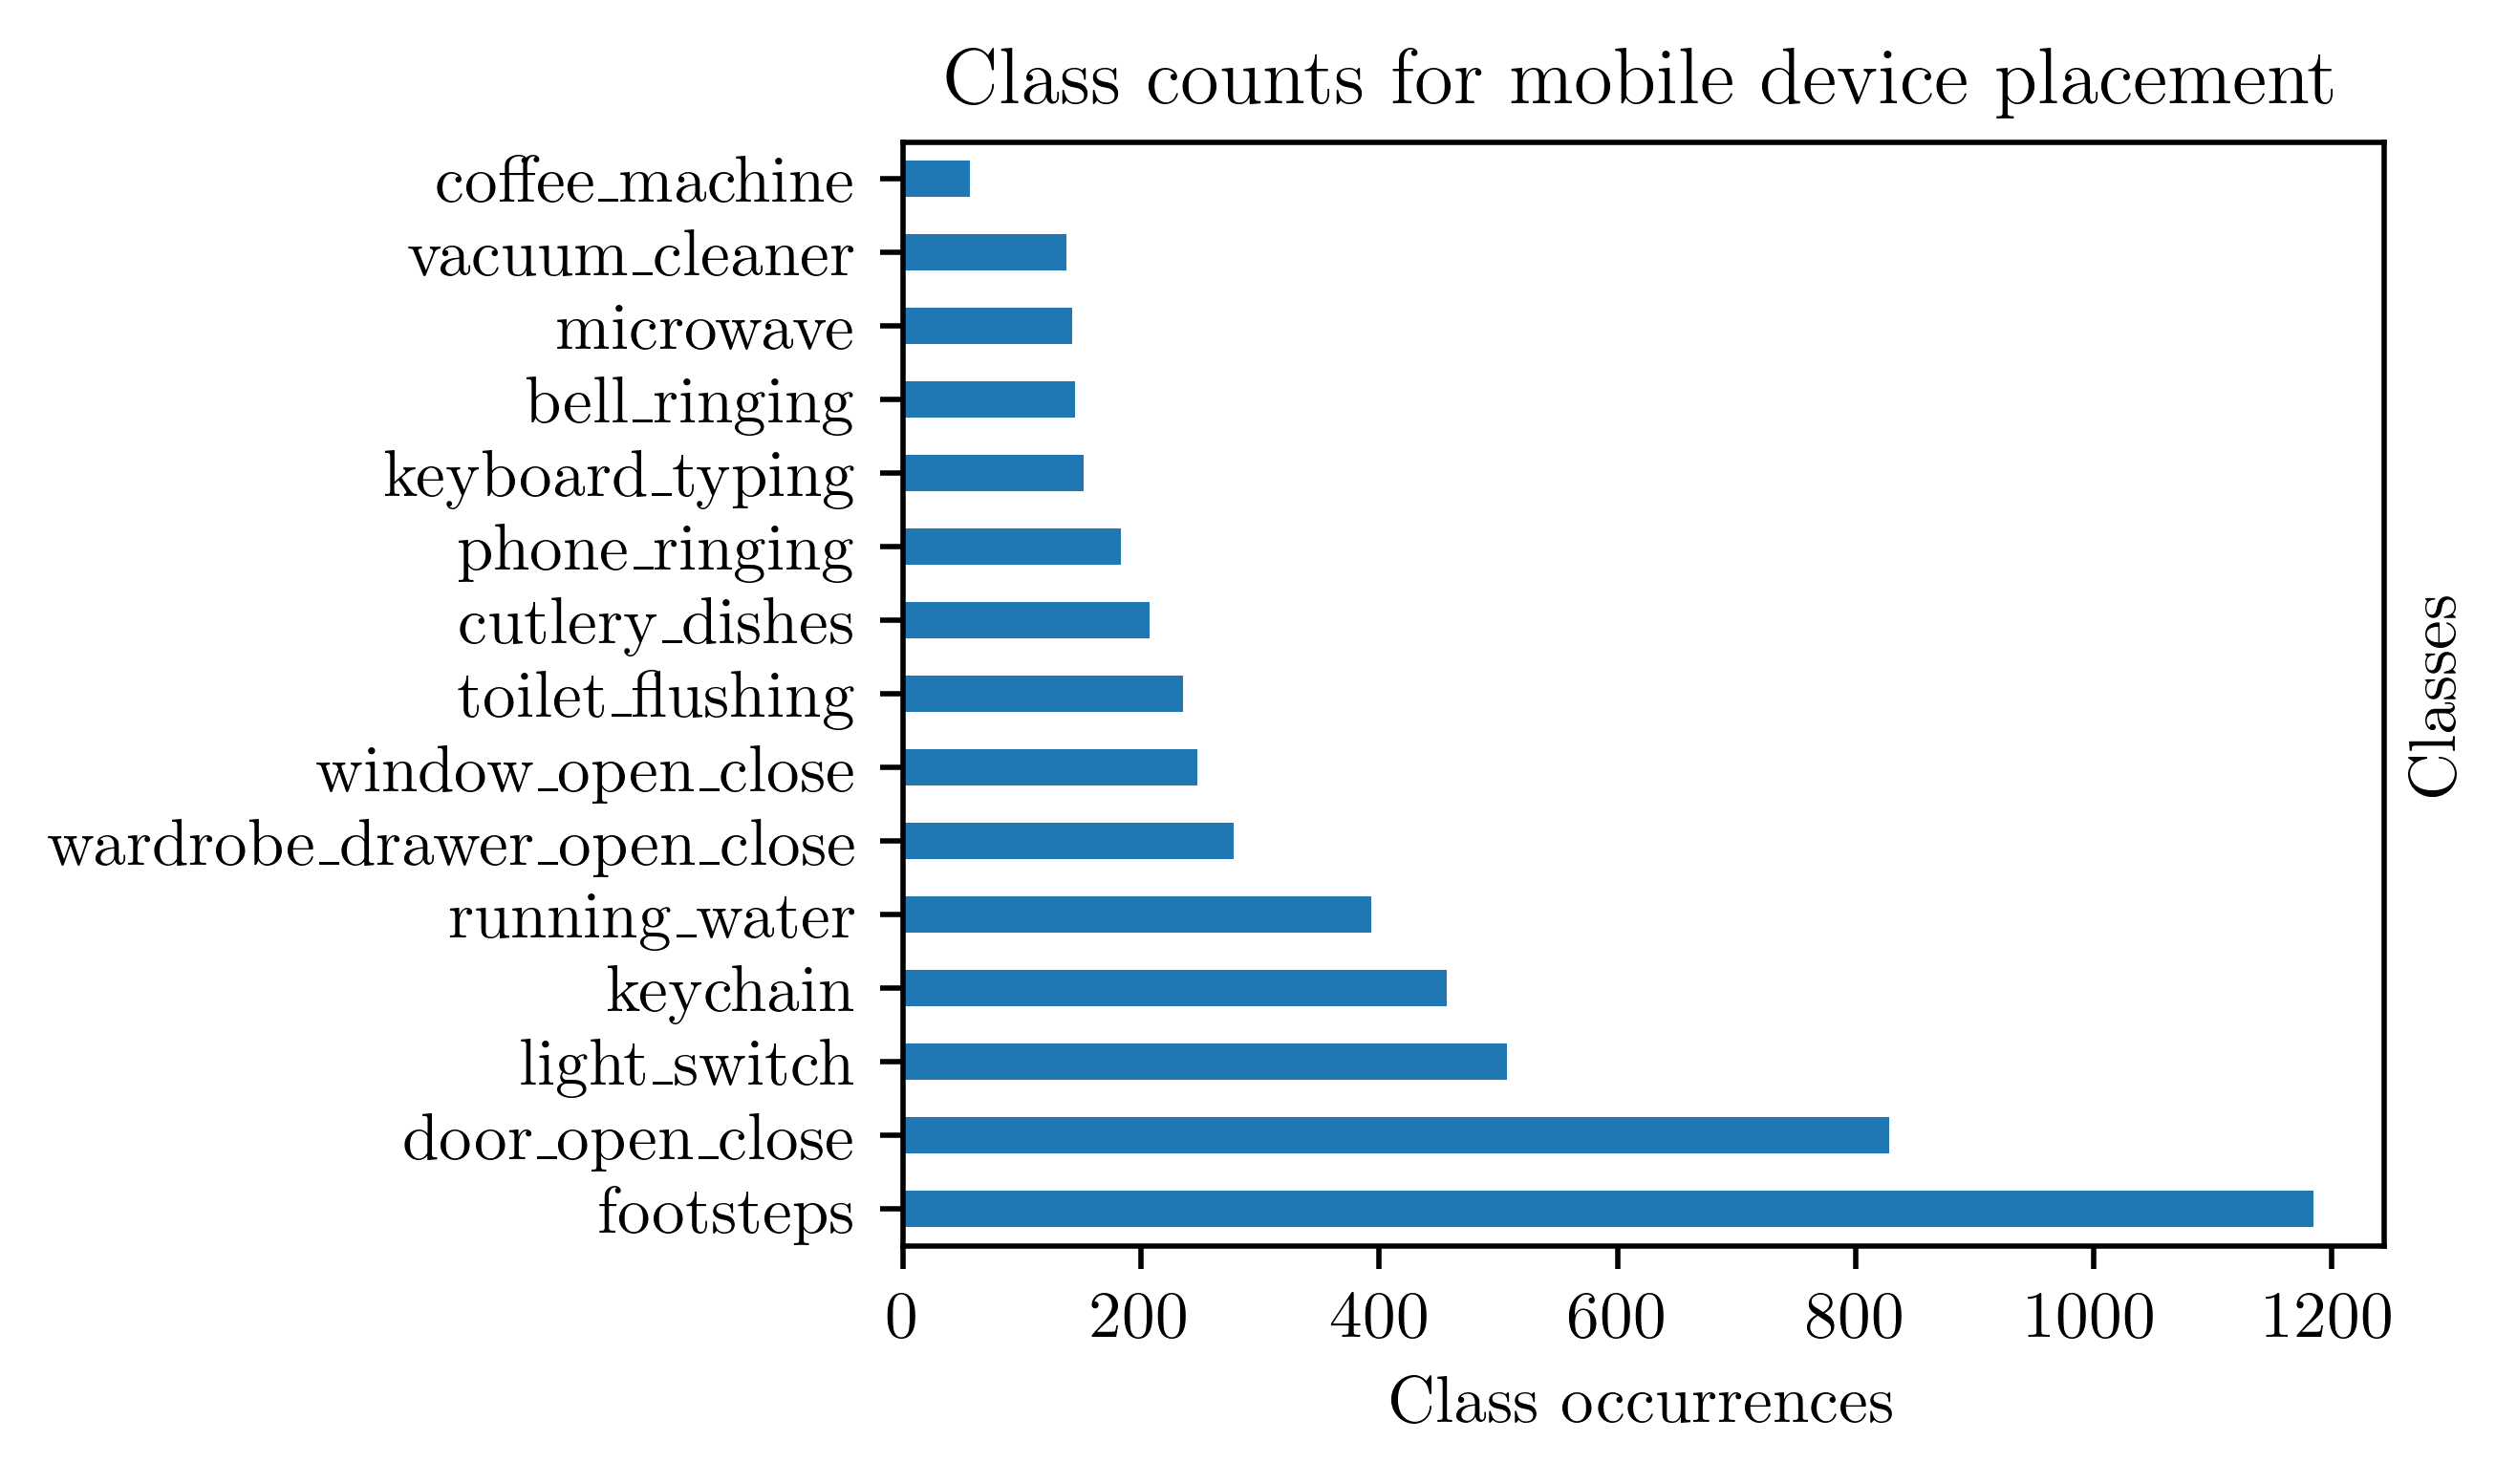
\includegraphics[width=\textwidth]{images/mobile-class-cnts.png}
        \caption{Number of classes with mobile device placement}\label{fig:placement-mobile}
    \end{subfigure}%
    \hfill
    \begin{subfigure}[t]{0.49\textwidth}
        \centering
        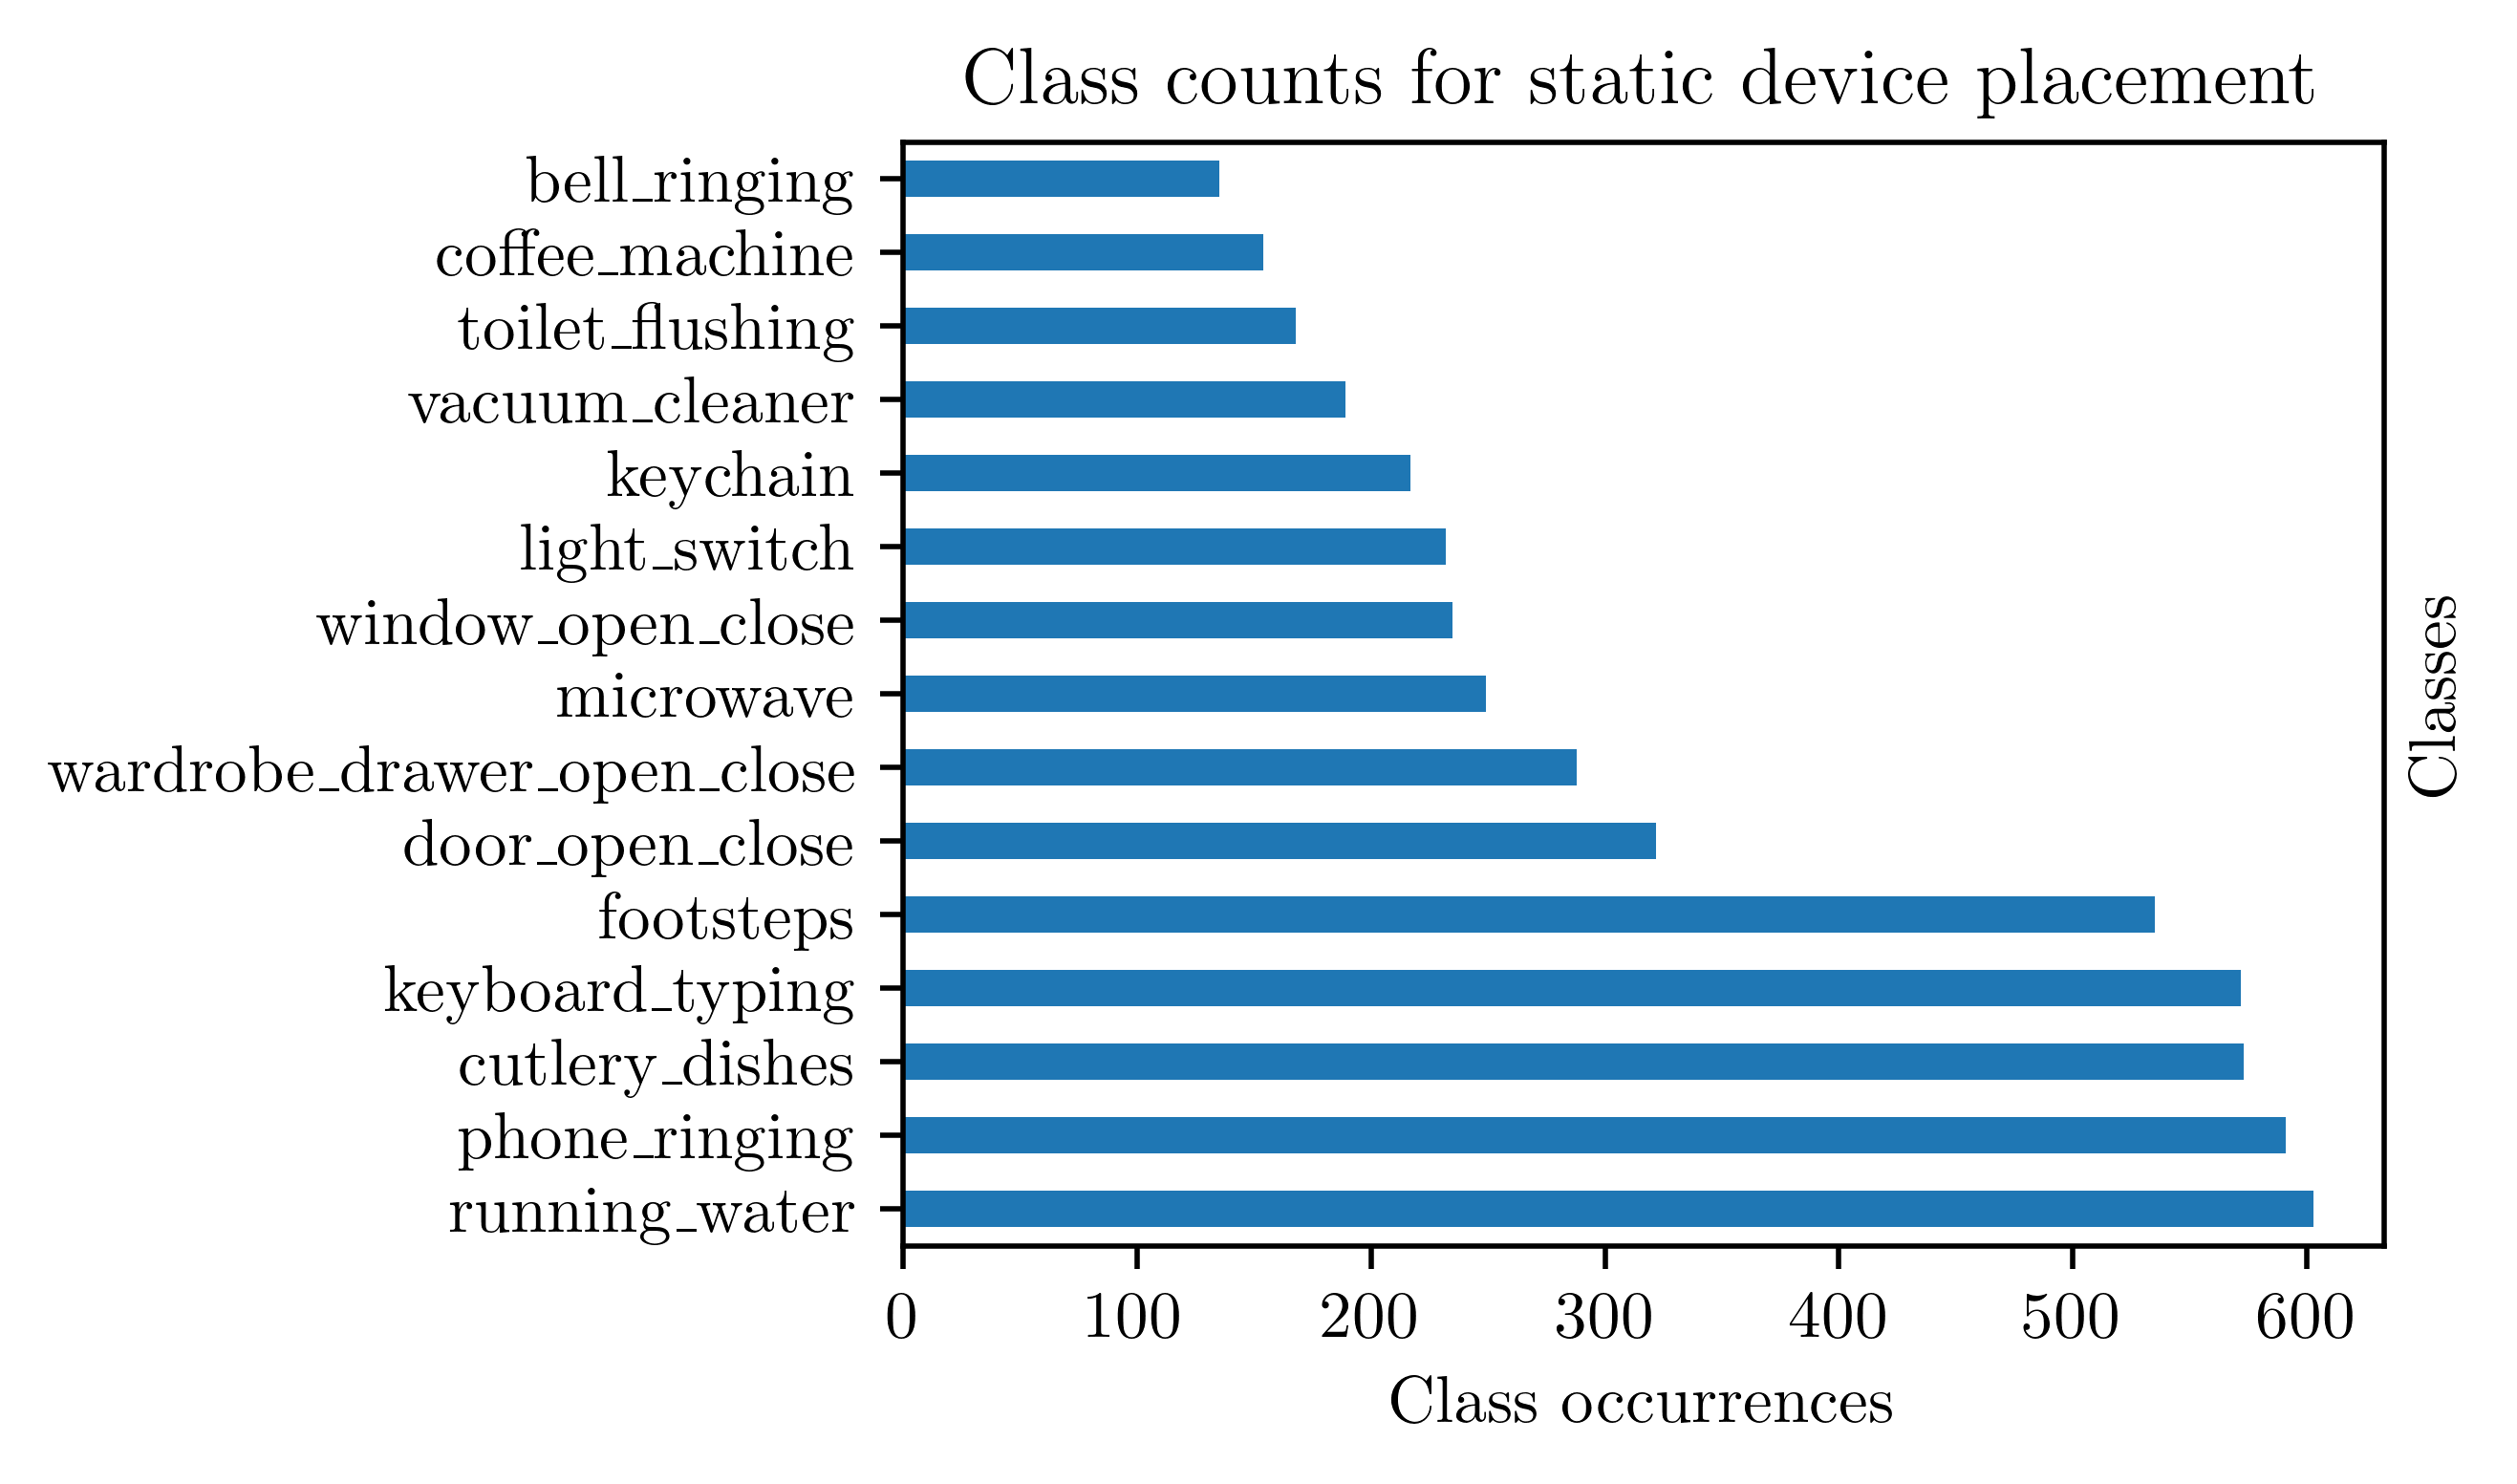
\includegraphics[width=\textwidth]{images/static-class-cnts.png}
        \caption{Number of classes with static device placement}\label{fig:placement-static}
    \end{subfigure}
    \caption{Comparison of class occurrences for recordings with mobile or static device placement}\label{fig:device-placement}
\end{figure}

\subsection{Feature Statistics}

\begin{wrapfigure}[10]{r}{0.4\textwidth}
    \raggedleft
    \vspace{-25pt}
    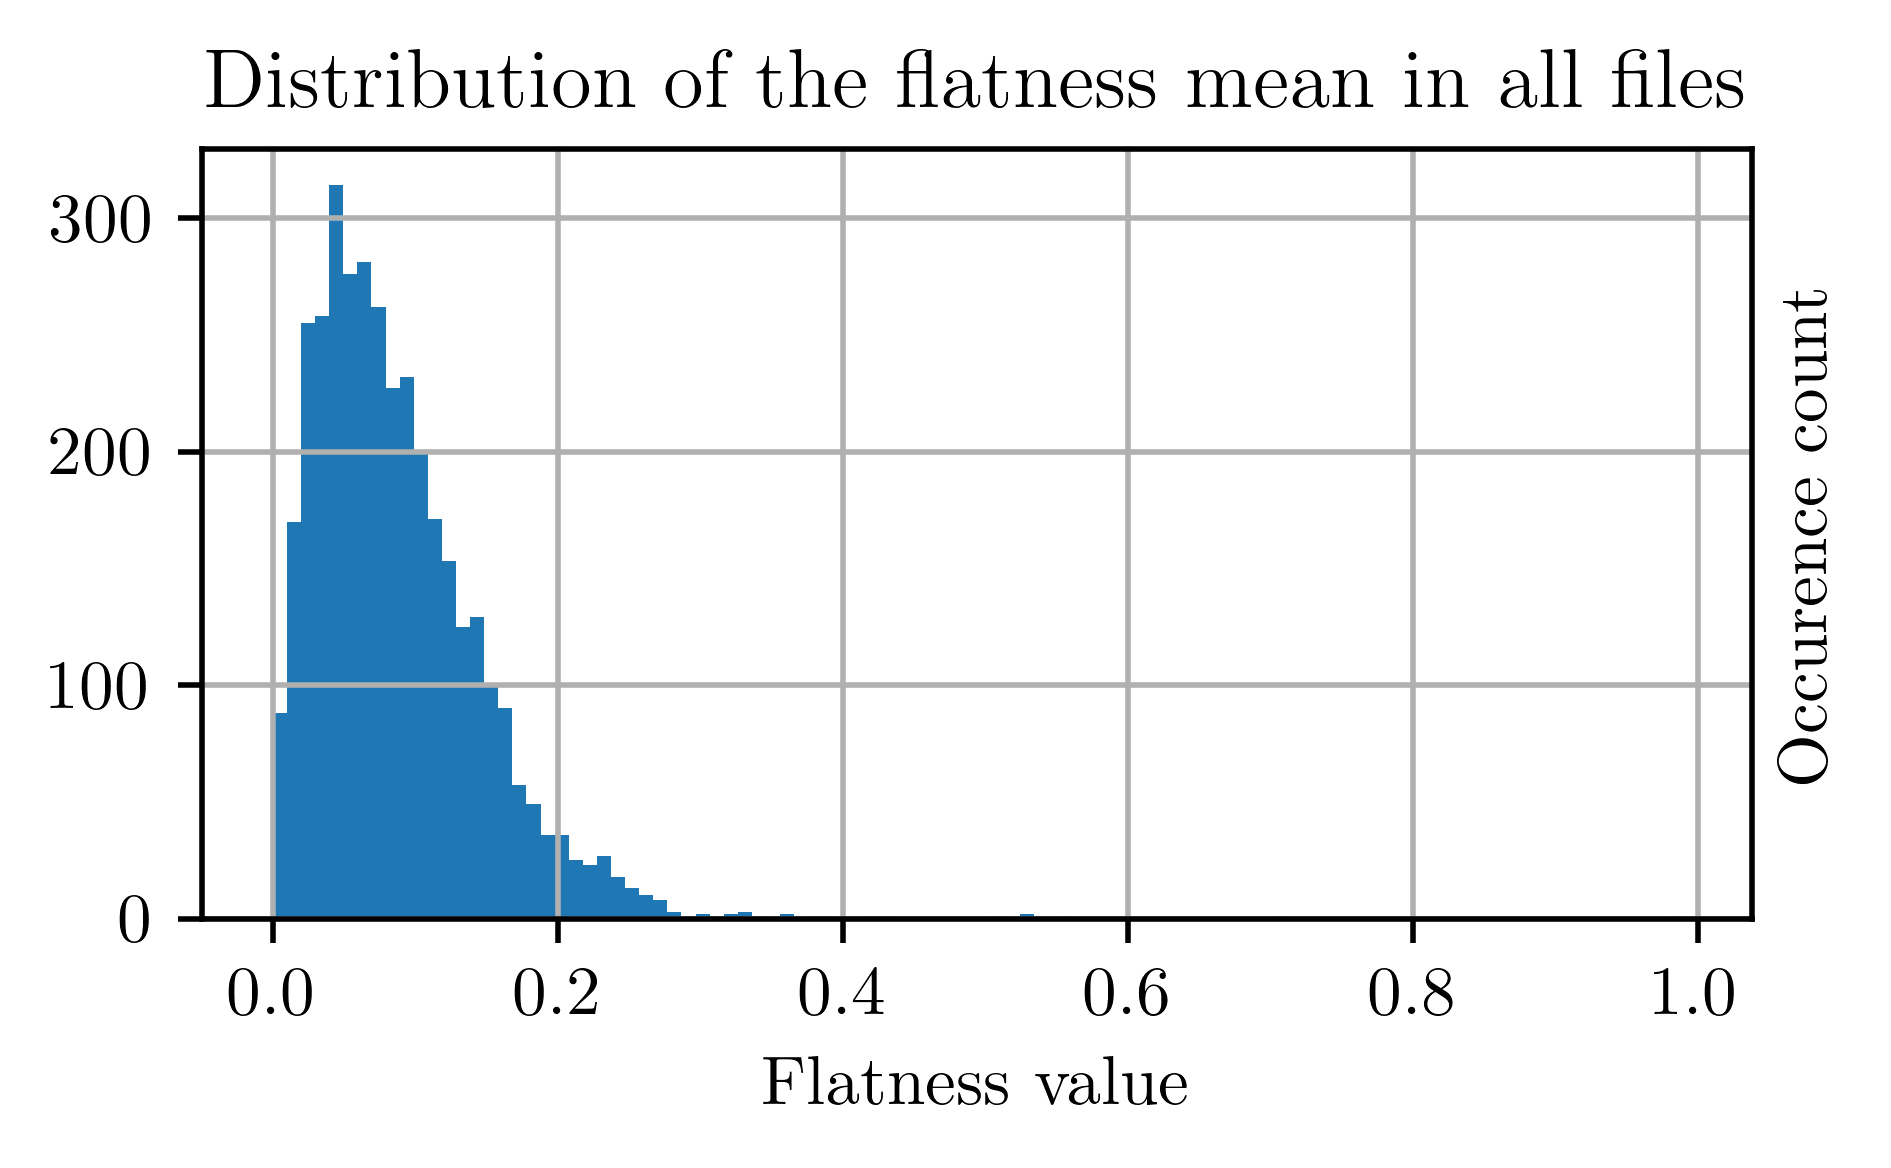
\includegraphics[width=0.35\textwidth]{images/flatness-dist.png}
    \caption{Distribution of the mean flatness value across all recordings}
    \label{fig:flatness-mean}
\end{wrapfigure}

The flatness of the spectrum will be closer examined. The flatness is a measure of how tonal a recording is. A value closer to $0.0$ means, that the energy is concentrated in individual frequencies, where as a value of $1.0$ indicates identical energy distribution to all frequency bins (= noise). \autoref{fig:flatness-mean} shows the distribution of the mean flatness of each file. High flatness values occur only in small amounts. These could stem from clothing rustle or similar.

\begin{itemize}
    \item Mean value: \si{0,0881}
    \item Standard deviation: \si{0,0616}
\end{itemize}

\subsection{Feature Correlation}

Upon comparing the audio features, it was noticed that the flatness is closely correlated with the bandwidth of the audio, which can be seen in \autoref{fig:flt-vs-bw}. This makes sense, as a more pure tone (equates to a low flatness value) does not need as much bandwidth as noise or signals with excessive harmonic content. Computing the correlation matrix \eqref{eq:corr-mtx} shows, that the flatness positively correlates with the bandwidth with a coefficient of \si{0,830}.

\begin{equation}
    \mathbf{R} = \begin{bmatrix}
        1 & \si{0,830} \\ \si{0,830} & 1
    \end{bmatrix}\label{eq:corr-mtx}
\end{equation}

\begin{figure}
    \centering
    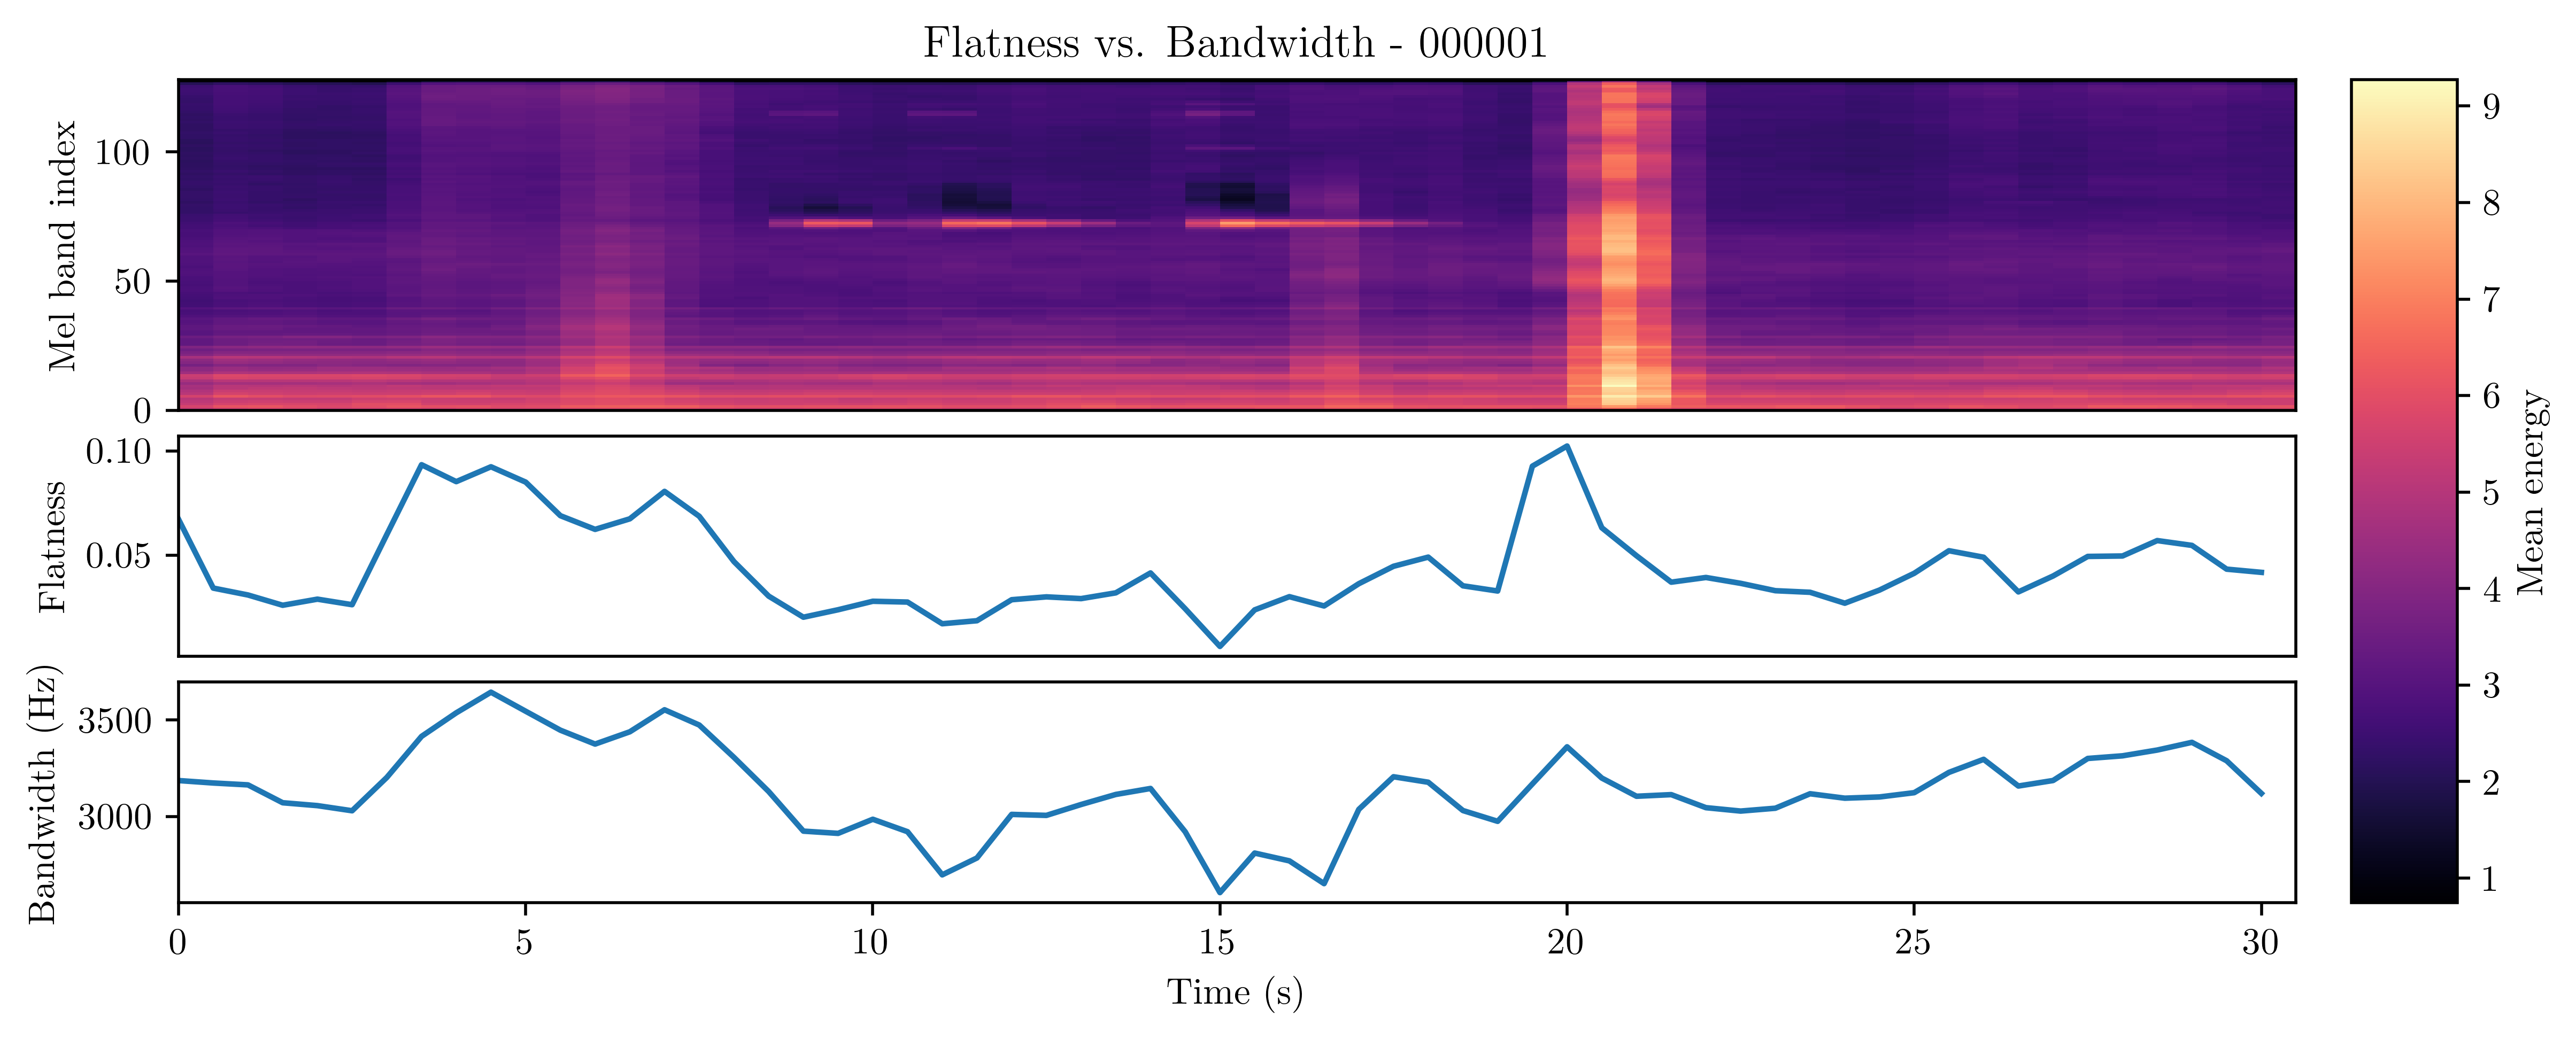
\includegraphics[width=0.8\textwidth]{flt-vs-bw.png}
    \caption{Comparison of the bandwidth and flatness feature with the Mel-Spectrum as a references}
    \label{fig:flt-vs-bw}
\end{figure}

\subsection{Feature Space Visualization}

To visualize the feature space in two dimensions, the dimensionality of the target class data has to be reduced. Two of the suggested methods are compared in \autoref{fig:feat-space}. UMAP (Uniform Manifold Approximation and Projection) preserves the global and local structure. Local clumps as well as the global shape is visible (\autoref{fig:umap}). t-SNE just retains the local structure, as only local clumps have structure, but the features are scattered on a global scale (\autoref{fig:tsne}).

\begin{figure}
\centering
\begin{subfigure}[c]{0.45\textwidth}
    \centering
    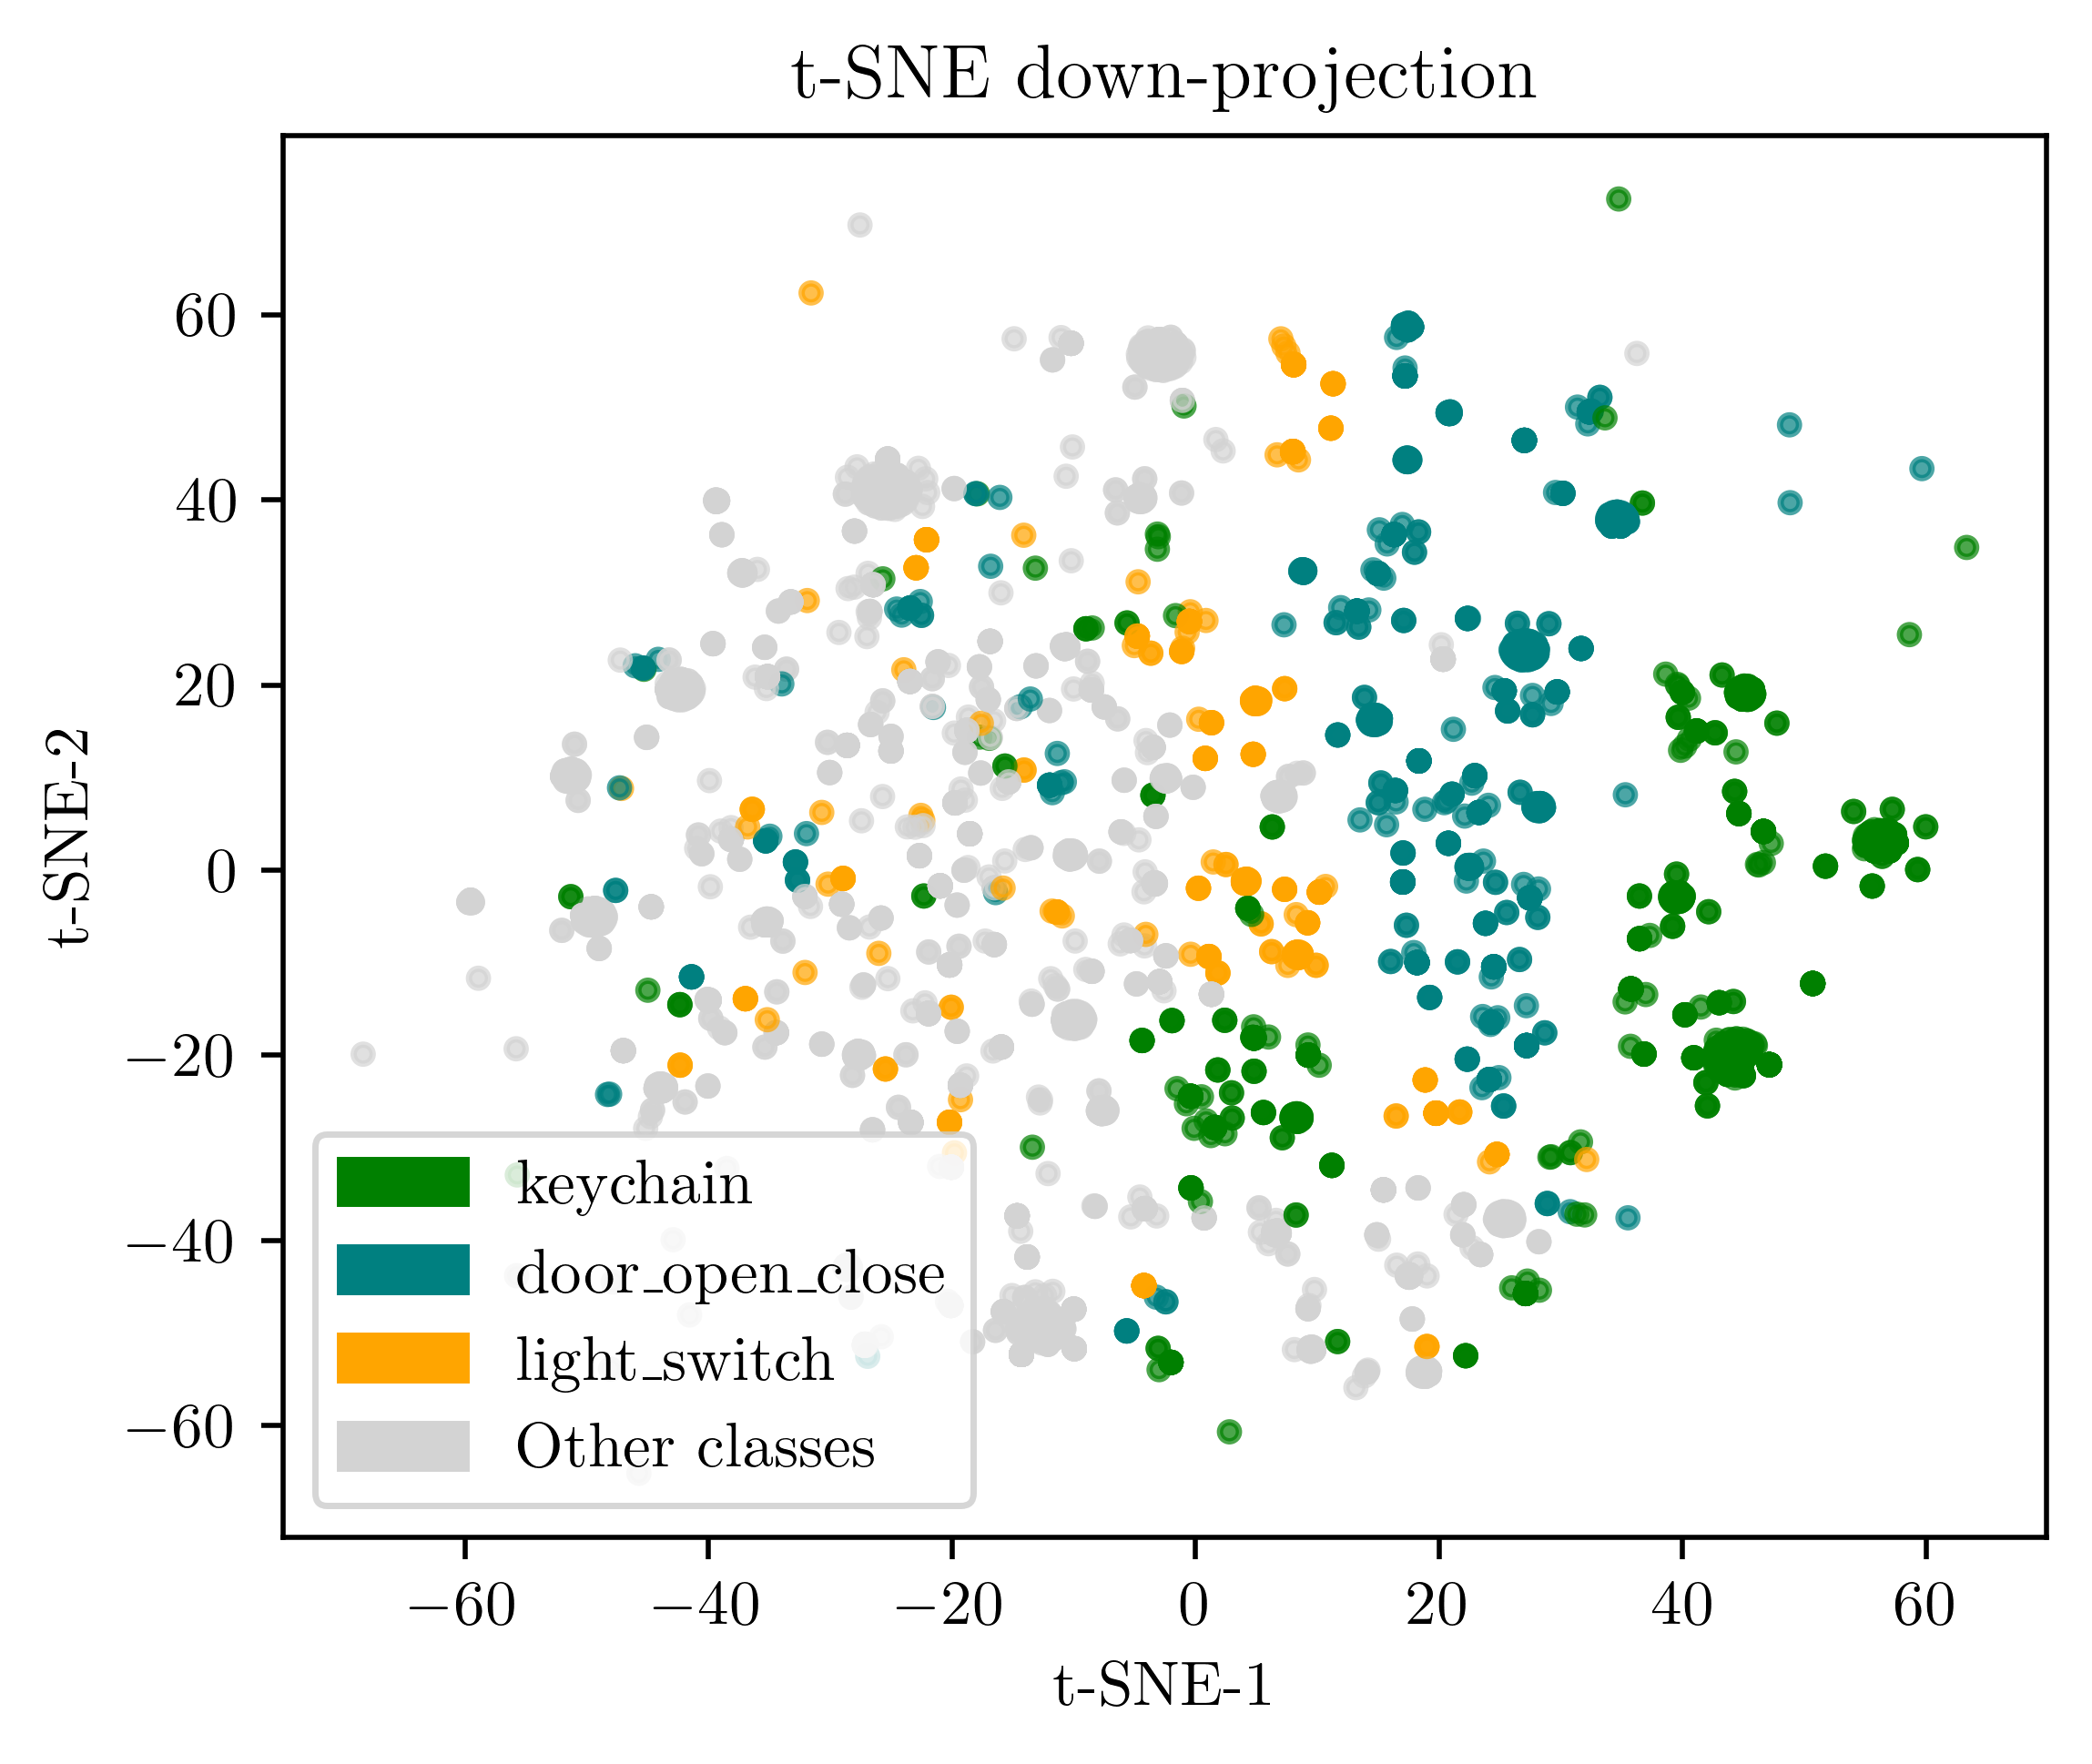
\includegraphics[width=\linewidth]{t-SNE-proj.png}
    \subcaption{t-SNE Method}
    \label{fig:tsne}
\end{subfigure}\hfill
\begin{subfigure}[c]{0.45\textwidth}
    \centering
    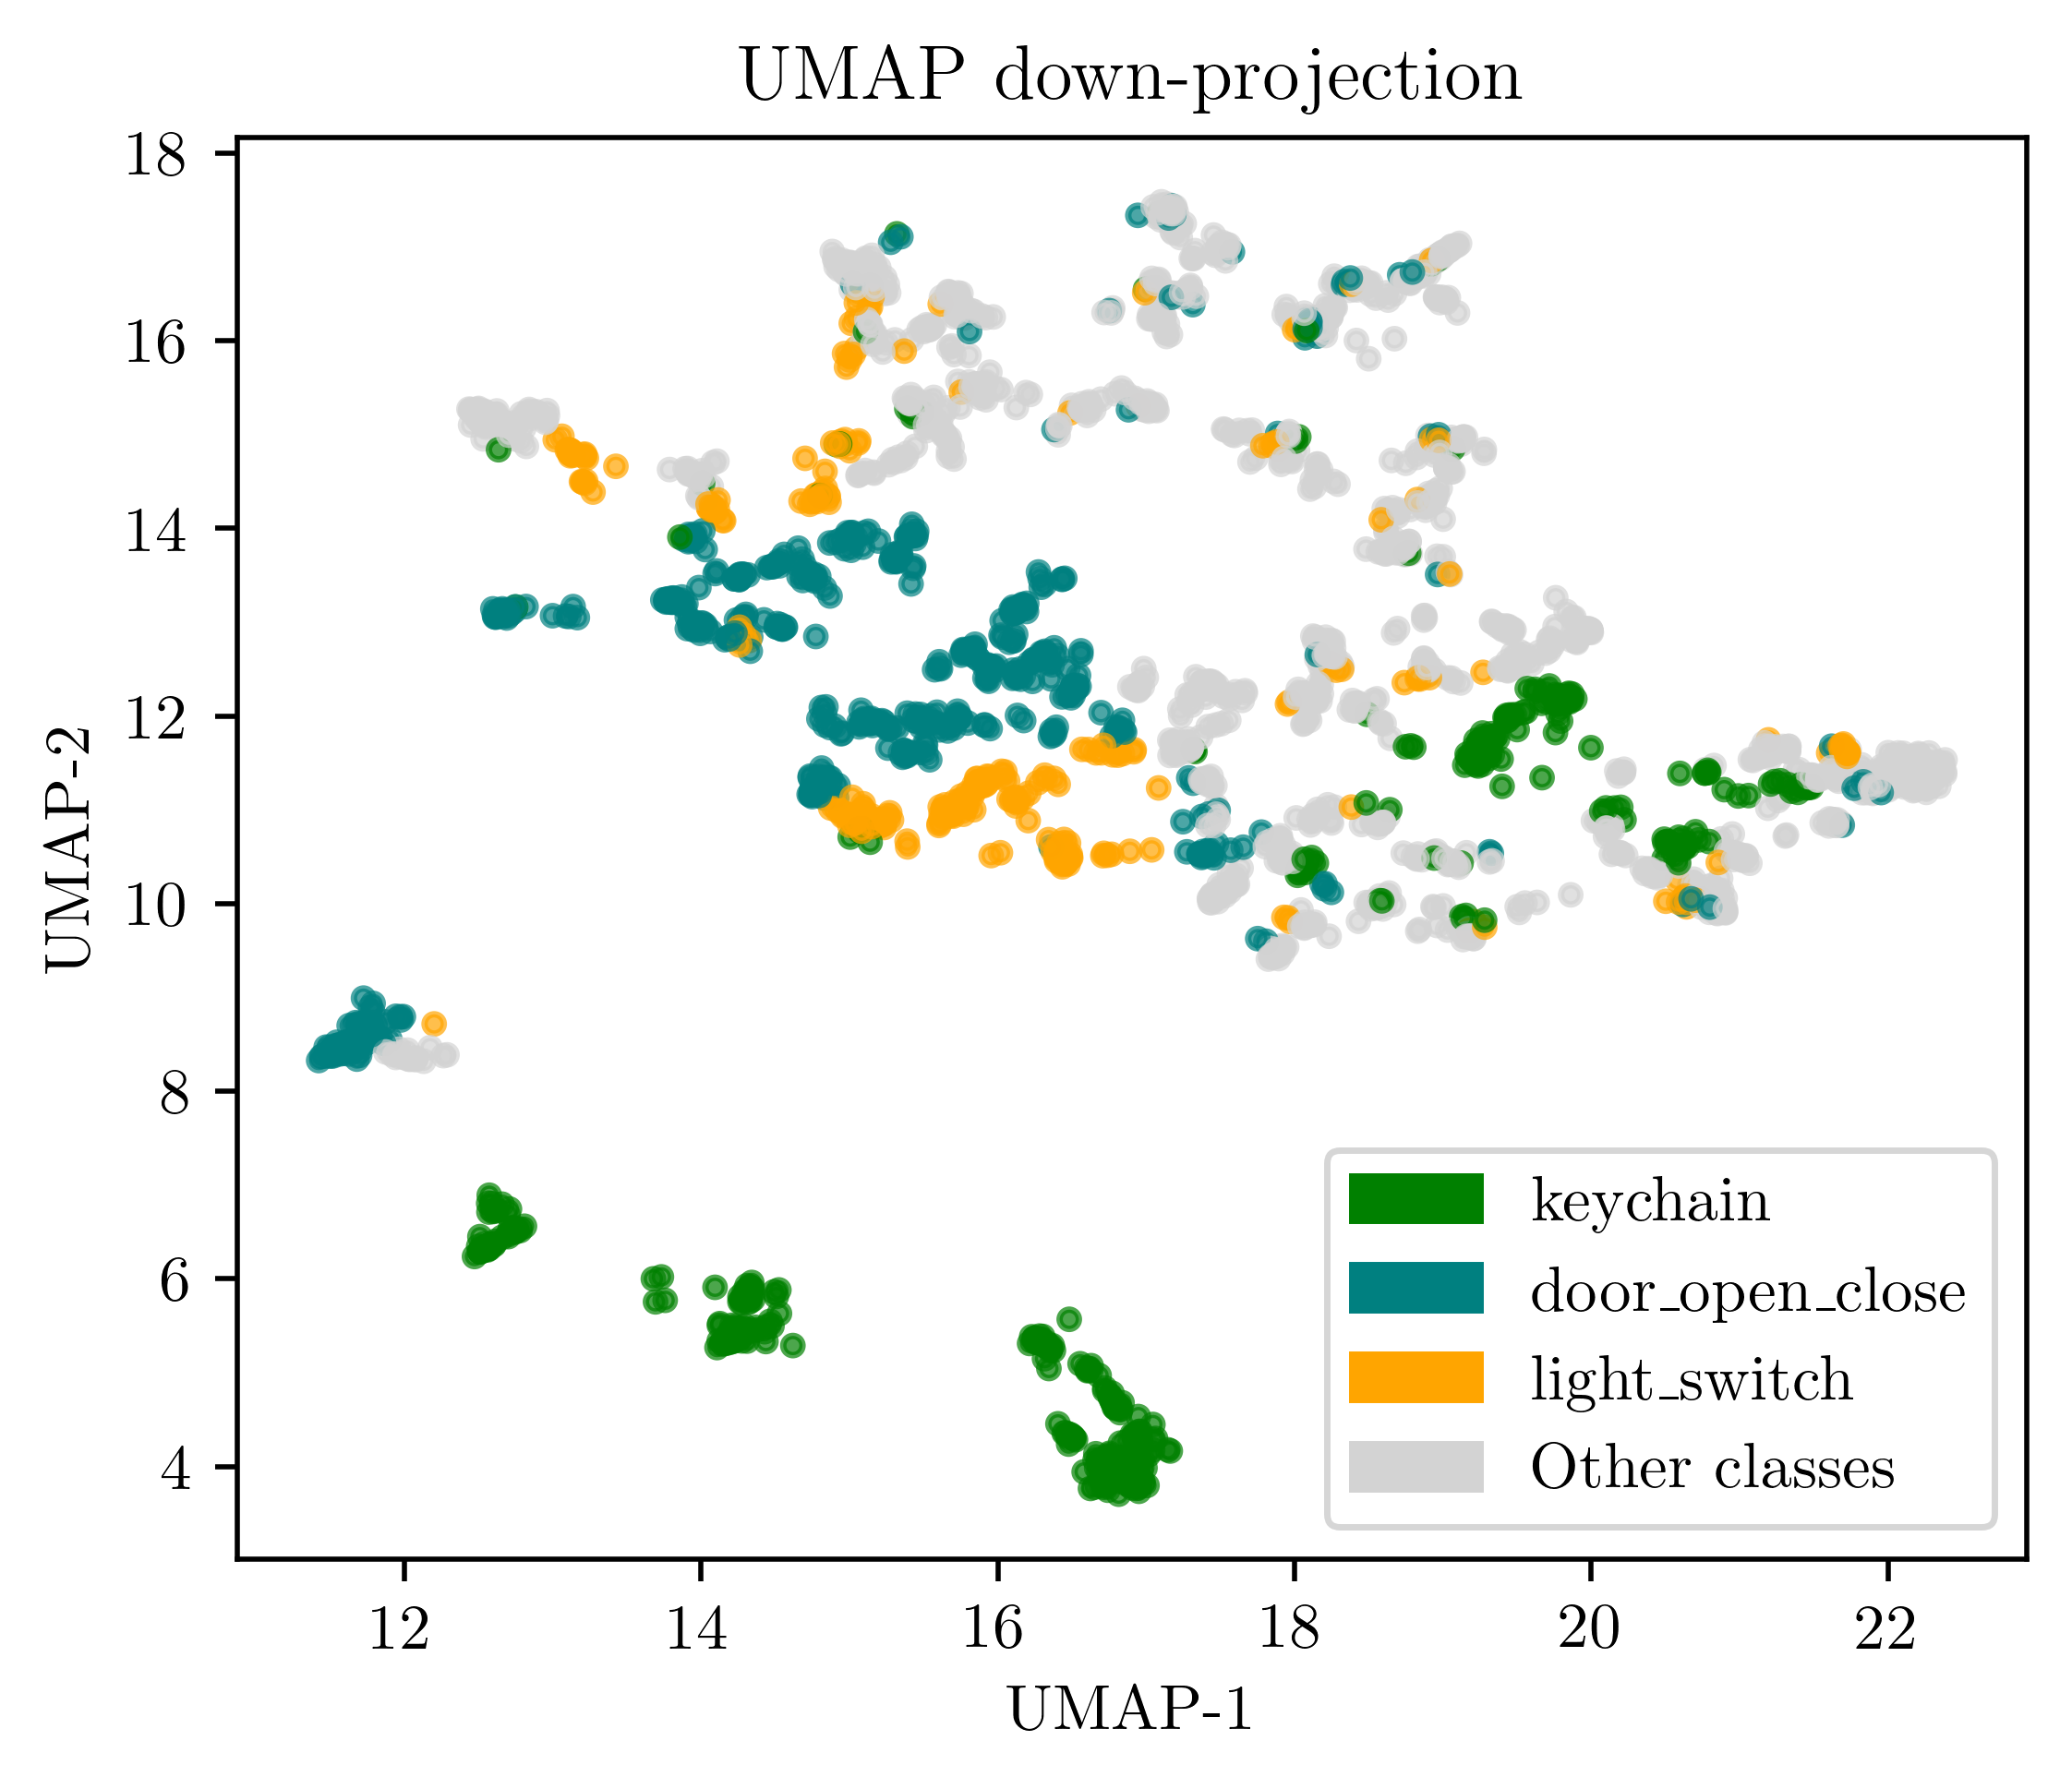
\includegraphics[width=\linewidth]{UMAP-proj.png}
    \subcaption{UMAP Method}\label{fig:umap}
\end{subfigure}
\caption{Visualization of the feature space using different down projection methods}\label{fig:feat-space}
\end{figure}

After trying out different hyper parameters to achieve a clear structure, the following were chosen:

\begin{itemize}
    \item \textbf{UMAP:} \lstinline{n_neigbors=30}, \lstinline{min_dist=0.1}
    \item \textbf{t-SNE:} \lstinline{perplexity=30} (default)
\end{itemize}

\section{Conclusion}

\paragraph{Biases}  Cases where annotator agreement is low have to be considered carefully. Different demographics and cultures may classify a "typical household" in different ways. Habits, routines and housing conditions affect the interpretation of scenarios. Additionally, classes are heavily imbalanced, so a model will likely favor common classes over rare ones. Around 17\% of files have only a single annotator, meaning their labels were never verified. Classes and recording environments are also correlated, so a model could learn room context as a shortcut rather than the actual sound.

\paragraph{Conclusion} Each recording stems from the soundscape of the everyday life of an individual, which might not share the habits of the annotator. For example a clicking sound right after a door opening would be interpreted as flicking a light switch, however it could also be a doorstop or the mechanism of the door itself. Hence, drawing the conclusion that the light is on after the occurrence of a clicking sound after a door was opened, does not hold true in the general case. Class imbalance and noisy labels for short events will make training challenging.

\paragraph{Broader Impact} Having a data set available online could help develop new applications for accessibility and safety in households. One of the places where accidents occur in the highest rate is the personal household. A sound detection system could help identify when an accident happens by detecting sounds from falls or broken glass, and for example call for help. 

However, the development of these applications raises the concern that technological advancements will lead to the normalization of surveillance. Renting an apartment in the future, where these systems might be implemented as a security standard or even enforced by law, is not acceptable for everyone.

Ethical use could be promoted by analyzing the data carefully such that no personal information is leaked and anonymity is ensured. Choosing a license at the beginning of the data collection was already a measure taken care of. Choosing the correct license could prevent proprietary use and selling information.

\section{Disclosure of LLM and AI Tool Use}

LLM was used to help with the transformation of pandas data frames and formatting plots. Support was also used to help understand how hyper-parameters of the projection methods are optimally chosen. LLM was also used for debugging code for the label conversion and label statistics, and for refining the clarity of some written paragraphs. All outputs were verified against the actual dataset.

%%%%%%%%%%%%%%%%%%%%%%%%%%%%%%%%%%%%%%%%%%%%%%%%%%%%%%%%%%%%

\end{document}